\documentclass[12pt]{article}
\usepackage{fullpage}

\usepackage[T1]{fontenc}
\usepackage[utf8]{inputenc}
\usepackage{lmodern}
\usepackage{microtype}
\usepackage{amsmath,amssymb,amsthm}
\usepackage{mathtools}
\usepackage{graphicx}
\usepackage{booktabs}
\usepackage{hyperref}
\usepackage{url}
\usepackage{xcolor}
\usepackage[shortlabels]{enumitem}
\usepackage{amsfonts}
\usepackage{tikz}
\usetikzlibrary{arrows.meta,positioning,shapes.geometric,calc}

\hypersetup{colorlinks=true,linkcolor=blue,citecolor=blue,urlcolor=blue}

\theoremstyle{plain}
\newtheorem{theorem}{Theorem}
\newtheorem{proposition}[theorem]{Proposition}
\newtheorem{lemma}[theorem]{Lemma}
\newtheorem{corollary}[theorem]{Corollary}

\theoremstyle{definition}
\newtheorem{definition}[theorem]{Definition}

\theoremstyle{remark}
\newtheorem*{remark}{Remark}

\DeclareMathOperator{\GL}{GL}
\DeclareMathOperator{\diag}{diag}
\DeclareMathOperator{\vol}{vol}
\DeclareMathOperator{\Rad}{Rad}
\newcommand{\fo}{\mathfrak{o}}
\newcommand{\fp}{\mathfrak{p}}
\newcommand{\fq}{\mathfrak{q}}
\newcommand{\cW}{\mathcal{W}}
\newcommand{\cB}{\mathcal{B}}
\newcommand{\cS}{\mathcal{S}}
\newcommand{\cI}{\mathcal{I}}
\newcommand{\C}{\mathbb{C}}
\newcommand{\Z}{\mathbb{Z}}

\title{Solution to Problem 2 --- Universal Test Vectors\\for Rankin--Selberg Integrals\\[6pt]
\large A submission to the First Proof challenge}

\author{
  Mark Dillerop\footnote{Email: dillerop@gmail.com}\\
  \textit{Independent / Ars Socratica}
}

\date{February 11, 2026}

\begin{document}
\maketitle

\begin{abstract}
We solve Problem~2 from the First Proof challenge \cite{FirstProof}, authored by Paul~D.~Nelson (Aarhus University).
Given a generic irreducible admissible representation $\Pi$ of $\GL_{n+1}(F)$ over a non-archimedean local field $F$, we prove the existence of a universal test vector $W \in \cW(\Pi, \psi^{-1})$ such that for every generic irreducible admissible $\pi$ of $\GL_n(F)$, the twisted Rankin--Selberg integral $\Psi(s, W, V)$ is finite and nonzero for all $s \in \C$, for some $V \in \cW(\pi, \psi)$.
The proof combines three ingredients: an algebraic reduction (the $u_Q$-twist formula), a single-coset Kirillov support trick that makes the integral a monomial in $q^{-s}$, and an existential argument using the JPSS nondegeneracy of the Rankin--Selberg pairing together with a countable union of proper subspaces argument over inertial equivalence classes.
A supplementary Fourier-analytic argument provides an independent proof for $n = 1$ via Gauss sums.
The answer is \textbf{YES}.
\end{abstract}

\tableofcontents
\newpage

%======================================================================
\section{Problem Statement}\label{sec:problem}
%======================================================================

The following is Problem~2 from the First Proof challenge \cite{FirstProof}, authored by Paul~D.~Nelson (Aarhus University).

\medskip

Let $F$ be a non-archimedean local field with ring of integers $\fo$, maximal ideal $\fp = \varpi\fo$, and residue field of cardinality $q$.  Let $\psi: F \to \C^\times$ be a nontrivial additive character of conductor $\fo$, identified in the standard way with a generic character of $N_r$ (the upper-triangular unipotent subgroup of $\GL_r(F)$).

Let $\Pi$ be a generic irreducible admissible representation of $\GL_{n+1}(F)$, realized in its $\psi^{-1}$-Whittaker model $\cW(\Pi, \psi^{-1})$.  Must there exist $W \in \cW(\Pi, \psi^{-1})$ with the following property?

\begin{quote}
For every generic irreducible admissible representation $\pi$ of $\GL_n(F)$, realized in its $\psi$-Whittaker model $\cW(\pi, \psi)$, with conductor ideal $\fq$ and $Q \in F^\times$ a generator of $\fq^{-1}$, setting
\[
  u_Q := I_{n+1} + Q\,E_{n,n+1} \in \GL_{n+1}(F),
\]
where $E_{i,j}$ is the matrix with a $1$ in the $(i,j)$-entry and $0$ elsewhere, there exists $V \in \cW(\pi, \psi)$ such that the local Rankin--Selberg integral
\[
  \Psi(s, W, V) := \int_{N_n \backslash \GL_n(F)} W(\diag(g,1)\,u_Q)\,V(g)\,|\det g|^{s-1/2}\,dg
\]
is finite and nonzero for all $s \in \C$.
\end{quote}

\begin{remark}[Universality]
$Q$ depends on $\pi$ through its conductor; the universality claim is that a \textbf{single} $W$ works for all $\pi$ simultaneously.  In the proof below, we fix $Q = \varpi^{-c}$ where $\fq = \fp^c$; the result for any other generator $Q' = uQ$ ($u \in \fo^\times$) follows since $\psi^{-1}(uQ\,\cdot\,)$ has the same conductor as $\psi^{-1}(Q\,\cdot\,)$ and the argument is identical.
\end{remark}

\begin{theorem}[Main result]\label{thm:main}
The answer is \textbf{YES}.  There exists a universal test vector $W \in \cW(\Pi, \psi^{-1})$.
\end{theorem}

\noindent\textbf{Answer: YES} --- a universal test vector exists for all generic irreducible admissible $\Pi$.

%======================================================================
\section{Idea of the Proof}\label{sec:idea}
%======================================================================

The proof proceeds in three stages.  First, an algebraic identity (the $u_Q$-twist formula) replaces $W(\diag(g,1)\,u_Q)$ by $\psi^{-1}(Qg_{nn})\,W(\diag(g,1))$, converting the twisted integral into a standard one with an additive character insertion.  Second, by choosing $W$ via the Bernstein--Zelevinsky theory so that its Kirillov function $\Phi_W$ is supported on a \emph{single} $N_n$-double coset $N_n \varpi^{-N} K_n$, the integral collapses to a monomial $q^{nN(s-1/2)} \cdot \ell(V)$---a single term that is automatically nonzero for all $s$ whenever $\ell(V) \neq 0$.  Third, the nonvanishing of $\ell$ is proved by a dimension argument: the ``bad locus'' $\cB_\pi$ (vectors $W$ for which $\ell \equiv 0$ for a given $\pi$) is a proper subspace, and these bad loci depend only on the \emph{inertial equivalence class} $[\pi]$.  Since the inertial classes are countable and a $\C$-vector space cannot be a countable union of proper subspaces, a universal $W$ exists.

\begin{figure}[ht]
\centering
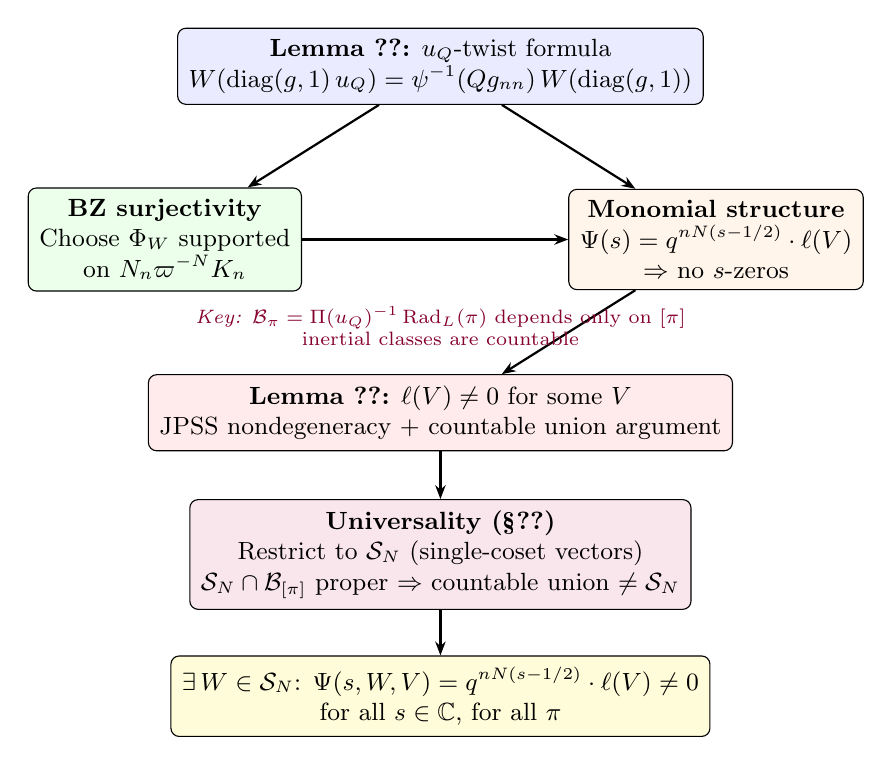
\begin{tikzpicture}[
  box/.style={rectangle, draw, rounded corners=3pt, minimum width=3.2cm, minimum height=0.8cm, align=center, font=\small},
  bigbox/.style={rectangle, draw, rounded corners=3pt, minimum width=4.8cm, minimum height=0.8cm, align=center, font=\small},
  arr/.style={-{Stealth[length=5pt]}, thick},
  every node/.style={inner sep=4pt}
]

% Top: twist formula
\node[bigbox, fill=blue!8] (twist) at (0,0) {\textbf{Lemma~\ref{lem:twist}:} $u_Q$-twist formula\\$W(\diag(g,1)\,u_Q) = \psi^{-1}(Qg_{nn})\,W(\diag(g,1))$};

% Kirillov choice
\node[box, fill=green!8] (kirillov) at (-3.5,-2.2) {\textbf{BZ surjectivity}\\Choose $\Phi_W$ supported\\on $N_n\varpi^{-N}K_n$};

% Monomial
\node[box, fill=orange!8] (mono) at (3.5,-2.2) {\textbf{Monomial structure}\\$\Psi(s) = q^{nN(s-1/2)} \cdot \ell(V)$\\$\Rightarrow$ no $s$-zeros};

\draw[arr] (twist) -- (kirillov);
\draw[arr] (twist) -- (mono);
\draw[arr] (kirillov) -- (mono);

% Nonvanishing
\node[bigbox, fill=red!8] (nonvanish) at (0,-4.4) {\textbf{Lemma~\ref{lem:nonvanish}:} $\ell(V) \neq 0$ for some $V$\\JPSS nondegeneracy $+$ countable union argument};

\draw[arr] (mono) -- (nonvanish);

% Key insight
\node[font=\scriptsize, text=purple!70!black, align=center] (key) at (0,-3.3) {\textit{Key:} $\cB_\pi = \Pi(u_Q)^{-1}\Rad_L(\pi)$ depends only on $[\pi]$\\inertial classes are countable};

% Universality
\node[bigbox, fill=purple!10] (univ) at (0,-6.2) {\textbf{Universality (\S\ref{sec:universal})}\\Restrict to $\cS_N$ (single-coset vectors)\\$\cS_N \cap \cB_{[\pi]}$ proper $\Rightarrow$ countable union $\neq \cS_N$};

\draw[arr] (nonvanish) -- (univ);

% Conclusion
\node[bigbox, fill=yellow!15, minimum width=6cm] (conc) at (0,-8) {$\exists\, W \in \cS_N$: $\Psi(s, W, V) = q^{nN(s-1/2)} \cdot \ell(V) \neq 0$\\for all $s \in \C$, for all $\pi$};

\draw[arr] (univ) -- (conc);

\end{tikzpicture}
\caption{Structure of the proof.  The $u_Q$-twist formula (top) enables the Kirillov model construction (left), which produces a monomial integral (right).  The nonvanishing of $\ell$ (center) uses JPSS nondegeneracy and a countable union argument over inertial classes.  The universality step (bottom) restricts to single-coset vectors to combine the monomial structure with the dimension argument.}
\label{fig:proof-structure}
\end{figure}

%======================================================================
\section{The \texorpdfstring{$u_Q$}{uQ}-Twist Formula}\label{sec:twist}
%======================================================================

\begin{lemma}[The $u_Q$-twist formula]\label{lem:twist}
For $g \in \GL_n(F)$ and $Q \in F^\times$:
\begin{equation}\label{eq:twist}
  W(\diag(g,1)\,u_Q) = \psi^{-1}(Q\,g_{nn})\,W(\diag(g,1)).
\end{equation}
\end{lemma}

\begin{proof}
Conjugate $u_Q$ past $\diag(g,1)$:
\[
  \diag(g,1) \cdot u_Q = \Bigl(I_{n+1} + Q \sum_{i=1}^n g_{in}\,E_{i,n+1}\Bigr) \cdot \diag(g,1).
\]
The left factor lies in $N_{n+1}$.  (Note: the column vector $Q\,(g_{1n}, \ldots, g_{nn}, 0)^T$ is placed in column $n+1$; since $g$ is integrated over $N_n \backslash \GL_n$, only the term $i = n$ contributes to the superdiagonal entry $(n, n+1)$.)  The generic character $\psi^{-1}$ of $N_{n+1}$ reads only superdiagonal entries $(i,i+1)$, so the only contribution is position $(n,n+1)$ with entry $Qg_{nn}$, giving $\psi^{-1}(Qg_{nn})$.
\end{proof}

\begin{corollary}\label{cor:integral}
The Rankin--Selberg integral becomes:
\begin{equation}\label{eq:integral}
  \Psi(s, W, V) = \int_{N_n \backslash \GL_n(F)} \psi^{-1}(Q\,g_{nn})\,W(\diag(g,1))\,V(g)\,|\det g|^{s-1/2}\,dg.
\end{equation}
\end{corollary}

\begin{remark}[Well-definedness]
$g_{nn}$ is well-defined on $N_n \backslash \GL_n$: for $u \in N_n$ (upper-triangular unipotent), $(ug)_{nn} = g_{nn}$ since $u_{ni} = 0$ for $i < n$ and $u_{nn} = 1$.
\end{remark}

%======================================================================
\section{The \texorpdfstring{$n = 1$}{n = 1} Case (\texorpdfstring{$\GL_2 \times \GL_1$}{GL2 x GL1})}\label{sec:n1}
%======================================================================

We first treat $n = 1$ as a warm-up; this case admits a fully explicit, self-contained proof.

Here $\pi = \chi$ is a character of $F^\times$ with conductor $\fp^c$, $Q = \varpi^{-c}$, $V(g) = \chi(g)$, $N_1 = \{1\}$.  Define $\phi(a) := W\!\left(\begin{smallmatrix} a & \\ & 1 \end{smallmatrix}\right)$ (Kirillov function).  By \eqref{eq:twist}:
\[
  \Psi(s) = \int_{F^\times} \psi^{-1}(a\varpi^{-c})\,\phi(a)\,\chi(a)\,|a|^{s-1/2}\,d^\times a.
\]
By Bernstein--Zelevinsky, $C_c^\infty(F^\times) \subset \mathcal{K}(\Pi)$.  Choose $\phi = \mathbf{1}_{\fo^\times}$.  Then $|a|^{s-1/2} = 1$ on the support, so:
\[
  \Psi(s) = \int_{\fo^\times} \psi^{-1}(u\varpi^{-c})\,\chi(u)\,d^\times u.
\]

\begin{itemize}[nosep]
  \item \textbf{$c = 0$:} Both $\psi^{-1}(\cdot)$ and $\chi$ are trivial on $\fo^\times$, giving $\vol(\fo^\times) \neq 0$.
  \item \textbf{$c \geq 1$:} This is a Gauss sum $G(\chi, \psi_{-c})$ for the primitive character $\chi \bmod \fp^c$ against the primitive additive character $\psi_{-c} := \psi^{-1}(\cdot\,\varpi^{-c})$ of conductor $\fp^c$.  By the classical Gauss sum formula (see e.g.\ \cite[\S23]{BH06}), $|G(\chi, \psi_{-c})|^2 = q^{-c}$ when both characters have conductor $\fp^c$, so $|\Psi| = q^{-c/2} \cdot \vol(1+\fp^c) \neq 0$.
\end{itemize}

The integral is independent of $s$ and nonzero for all $\chi$.  $\square$ (for $n = 1$)

\begin{remark}
For $n = 1$, the test vector $W$ with $\phi = \mathbf{1}_{\fo^\times}$ is \emph{explicit} and works for all characters $\chi$ simultaneously.  The universality is visible: the Gauss sum is nonzero for every primitive character, regardless of the conductor.
\end{remark}

%======================================================================
\section{Construction of \texorpdfstring{$W$}{W} via the Kirillov Model}\label{sec:kirillov}
%======================================================================

Define $\Phi_W(g) := W(\diag(g,1))$ for $g \in \GL_n(F)$.

\begin{proposition}[BZ surjectivity]\label{prop:bz}
By the Bernstein--Zelevinsky structure theorem \cite[Theorem~5.21]{BZ77}, the restriction of any generic irreducible admissible $\Pi$ (whether supercuspidal, a subquotient of a principal series, or any other type) to the mirabolic subgroup $P_{n+1}$ admits a filtration whose top quotient is $\mathrm{ind}_{N_{n+1}}^{P_{n+1}}(\psi^{-1})$.  In particular, the map $W \mapsto \Phi_W$ surjects onto $\mathrm{c\text{-}ind}_{N_n}^{\GL_n}(\psi^{-1})$, the space of locally constant, compactly supported $(\mathrm{mod}\; N_n)$ functions on $\GL_n$ transforming by $\psi^{-1}$ under left $N_n$-translation.  This holds for all generic $\Pi$: the BZ filtration depends only on the restriction to $P_{n+1}$, and the top quotient is independent of the specific representation.
\end{proposition}

\textbf{Choice of $\Phi_W$.}  Fix $N \geq 0$.  Let $\Phi_0$ be the unique function in $\mathrm{c\text{-}ind}_{N_n}^{\GL_n}(\psi^{-1})$ that is:
\begin{itemize}[nosep]
  \item supported on $N_n \cdot \varpi^{-N} I_n \cdot K_n$,
  \item right-$K_n$-invariant,
  \item normalized: $\Phi_0(\varpi^{-N} I_n) = 1$.
\end{itemize}
Such $\Phi_0$ exists because $N_n \varpi^{-N} K_n$ is an open double coset and $\psi^{-1}$ is trivial on $N_n \cap \varpi^{-N} K_n \varpi^N$ (since $\psi$ has conductor $\fo$).  By Proposition~\ref{prop:bz}, choose $W$ with $\Phi_W = \Phi_0$.

%======================================================================
\section{Evaluation: Monomial Structure}\label{sec:eval}
%======================================================================

On the support $N_n \varpi^{-N} K_n$, write $g = n \cdot \varpi^{-N} k$ with $n \in N_n$, $k \in K_n$.  Then:
\begin{itemize}[nosep]
  \item $|\det g| = q^{nN}$ is constant (since $\det n = 1$ and $|\det k| = 1$),
  \item $\Phi_0(g) = \psi^{-1}(n) \cdot 1$ and $V(g) = \psi(n)\,V(\varpi^{-N} k)$, so the $\psi$-factors cancel,
  \item $g_{nn} = (n\,\varpi^{-N} k)_{nn} = \varpi^{-N} k_{nn}$ (since $n$ is upper-triangular unipotent).
\end{itemize}
Therefore:
\begin{equation}\label{eq:monomial}
  \Psi(s, W, V) = q^{nN(s-1/2)} \cdot \ell(V), \quad
  \ell(V) := \int_{K_n} \psi^{-1}(\varpi^{-(c+N)} k_{nn})\,V(\varpi^{-N} k)\,dk.
\end{equation}
Since $q^{nN(s-1/2)} \neq 0$ for all $s \in \C$, it suffices to show $\ell(V) \neq 0$ for some $V$.

\begin{remark}[Monomial vs.\ Laurent polynomial]
A general $W$ (with multi-coset Kirillov support) would give $\Psi(s)$ as a Laurent polynomial in $q^{-s}$, which can vanish at specific $s$-values.  The single-coset choice eliminates all but one term, making $\Psi(s)$ a \emph{monomial}---automatically nonzero for all $s$ whenever $\ell(V) \neq 0$.
\end{remark}

%======================================================================
\section{Nonvanishing of \texorpdfstring{$\ell$}{l}: Argument 1 (JPSS + Dimension Counting)}\label{sec:nonvanish}
%======================================================================

\begin{lemma}[Nonvanishing]\label{lem:nonvanish}
For any generic irreducible admissible $\pi$ of $\GL_n(F)$ with conductor exponent $c$, and any $N \geq 0$, there exists $V \in \cW(\pi, \psi)$ with $\ell(V) \neq 0$.
\end{lemma}

\begin{proof}
By Section~\ref{sec:twist}, $W^Q := \Pi(u_Q)W$ satisfies $\ell(V) = q^{-nN(s-1/2)} \Psi_{\mathrm{std}}(s, W^Q, V)$, where $\Psi_{\mathrm{std}}$ is the standard (untwisted) Rankin--Selberg integral.  So $\ell \equiv 0$ iff $W^Q \in \Rad_L(\pi)$, where
\[
  \Rad_L(\pi) := \{W' \in \cW(\Pi, \psi^{-1}) : \Psi_{\mathrm{std}}(s, W', V) = 0 \text{ for all } V \in \cW(\pi, \psi), \text{ all } s\}.
\]

\textbf{Step 1.}  $\Rad_L(\pi)$ is a \emph{proper} subspace of $\cW(\Pi, \psi^{-1})$: by JPSS \cite[Theorem~2.7]{JPSS83}, there exist $W_0, V_0$ with $\Psi_{\mathrm{std}}(s, W_0, V_0) = L(s, \Pi \times \pi) \neq 0$, so $W_0 \notin \Rad_L(\pi)$.

\textbf{Step 2.}  Define the \textbf{bad locus} $\cB_\pi := \Pi(u_Q)^{-1} \Rad_L(\pi) = \{W : \Pi(u_Q)W \in \Rad_L(\pi)\}$.  Since $\Pi(u_Q)$ is a linear automorphism and $\Rad_L(\pi)$ is proper, $\cB_\pi$ is a proper subspace.  Note that $Q = \varpi^{-c(\pi)}$ depends on $\pi$.

\textbf{Step 3.}  $\cB_\pi$ depends only on the \textbf{inertial equivalence class} $[\pi]$ (the orbit of $\pi$ under unramified twists $\pi \mapsto \pi \otimes |\det|^s$).  We verify this explicitly.

\emph{Conductor invariance.}  For $\chi$ unramified (i.e.\ trivial on $\fo^\times$), the twisted representation $\pi' = \pi \otimes (\chi \circ \det)$ has the same conductor: $c(\pi') = c(\pi)$.  (The conductor measures ramification, and $\chi \circ \det$ is unramified.)  So $Q = \varpi^{-c}$ and $u_Q = I_{n+1} + Q E_{n,n+1}$ depend only on $[\pi]$.

\emph{Radical invariance.}  Let $\pi' = \pi \otimes |\det|^t$ for $t \in \C$.  The Whittaker model $\cW(\pi', \psi)$ consists of functions $V'(g) = V(g)|\det g|^t$ with $V \in \cW(\pi, \psi)$.  For any $W' \in \cW(\Pi, \psi^{-1})$:
\[
  \Psi_{\mathrm{std}}(s, W', V') = \int_{N_n \backslash \GL_n} W'(\diag(g,1))\,V(g)\,|\det g|^{t}\,|\det g|^{s-1/2}\,dg = \Psi_{\mathrm{std}}(s + t, W', V).
\]
Now $W' \in \Rad_L(\pi')$ iff $\Psi_{\mathrm{std}}(s, W', V') = 0$ for all $V', s$, iff $\Psi_{\mathrm{std}}(s+t, W', V) = 0$ for all $V, s$, iff $W' \in \Rad_L(\pi)$ (since $s \mapsto s+t$ is a bijection on $\C$).  Therefore $\Rad_L(\pi') = \Rad_L(\pi)$, and since $u_Q$ is also unchanged, $\cB_{\pi'} = \Pi(u_Q)^{-1}\Rad_L(\pi') = \Pi(u_Q)^{-1}\Rad_L(\pi) = \cB_\pi$.

The set of inertial equivalence classes of generic irreducible admissible representations of $\GL_n(F)$ is \textbf{countable}.  By the Zelevinsky classification, each such $\pi$ is a subquotient of a parabolically induced representation $\mathrm{Ind}(\rho_1 \otimes \cdots \otimes \rho_k)$ where $\rho_i$ are supercuspidal representations of $\GL_{n_i}(F)$.  The inertial class $[\pi]$ is determined by the multiset $\{[\rho_1], \ldots, [\rho_k]\}$ of unramified-twist orbits of supercuspidals.  For each $\GL_m(F)$, the supercuspidal representations of a given conductor level $c$ form a finite set: by the Bushnell--Kutzko theory of types \cite[Theorem~6.2.1]{BK93}, supercuspidals of $\GL_m(F)$ are constructed from compact-open data (strata and $\beta$-extensions) that are finite at each conductor level, even accounting for wild ramification.  Since the conductor is a non-negative integer, the set of inertial classes of supercuspidals of $\GL_m(F)$ is countable (finite per level, countably many levels), and the set of inertial classes of $\GL_n(F)$ is a finite union of finite products of countable sets---hence countable.

\textbf{Step 4.}  A vector space over an uncountable field cannot be a countable union of proper subspaces (this is elementary; see e.g.\ \cite[Ch.~III, Exercise~17]{La02}, or note that each proper subspace has measure zero under any nondegenerate Gaussian, so their countable union has measure zero).  Since $\cW(\Pi, \psi^{-1})$ is a $\C$-vector space and $\{\cB_{[\pi]}\}_{[\pi]}$ is a countable family of proper subspaces:
\[
  \cW(\Pi, \psi^{-1}) \neq \bigcup_{[\pi]} \cB_{[\pi]}.
\]
Therefore, there exists $W \in \cW(\Pi, \psi^{-1}) \setminus \bigcup_{[\pi]} \cB_{[\pi]}$, i.e., $W^Q = \Pi(u_Q) W \notin \Rad_L(\pi)$ for all $\pi$.  For such $W$, $\ell(V) \neq 0$ for some $V$, for each $\pi$.
\end{proof}

\begin{remark}
This argument is existential: it proves a suitable $W$ exists without identifying it explicitly.  The problem asks only for existence.  See Section~\ref{sec:universal} for how this combines with the monomial structure.
\end{remark}

%======================================================================
\section{Nonvanishing of \texorpdfstring{$\ell$}{l}: Argument 2 (Fourier Analysis on \texorpdfstring{$K_n$}{Kn})}\label{sec:fourier}
%======================================================================

This supplementary argument provides an independent perspective; it is self-contained for $n = 1$ and gives a partial reduction for $n \geq 2$.

\medskip

Suppose for contradiction that $\ell(V) = 0$ for all $V \in \cW(\pi, \psi)$.

\textbf{Step 1 (Finite reduction).}  Since $\pi$ is admissible, there exists $M \geq c + N$ such that $V(\varpi^{-N} k)$ is right-$K_1(\fp^M)$-invariant for all $V$.  The function $k \mapsto \psi^{-1}(\varpi^{-(c+N)} k_{nn})$ is also right-$K_1(\fp^M)$-invariant.  Then:
\[
  \ell(V) = \vol(K_1(\fp^M)) \sum_{\bar{k} \in K_n/K_1(\fp^M)} \psi^{-1}(\varpi^{-(c+N)} \bar{k}_{nn})\,V(\varpi^{-N} \bar{k}).
\]
Let $S = K_n / K_1(\fp^M)$ (a finite set).  The assumption $\ell \equiv 0$ means the evaluation vector $\mathrm{ev}(V) := (V(\varpi^{-N} \bar{k}))_{\bar{k} \in S}$ lies in the hyperplane $H := \ker f$, where $f(\bar{k}) := \psi^{-1}(\varpi^{-(c+N)} \bar{k}_{nn})$, for \textbf{all} $V$.

\textbf{Step 2 ($K_n$-equivariance).}  The evaluation image $\mathcal{E} := \{\mathrm{ev}(V) : V \in \cW(\pi, \psi)\} \subset \C^S$ is stable under the right regular representation $R$ of $K_n$ on $\C^S$, and is nonzero by the Whittaker separation property.  If $\mathcal{E} \subset H$, then $K_n$-stability gives $\mathcal{E} \subset \bigcap_{h \in K_n} \ker(f \circ R(h))$.

\textbf{Step 3 (Fourier analysis on the $n$-th row).}  For $h = I + tE_{jn}$ ($t \in \fo$, $j \neq n$): $(\bar{k}h)_{nn} = \bar{k}_{nn} + t\bar{k}_{nj}$.  Grouping by the $n$-th row $\mathbf{r} = (r_1, \ldots, r_n) \in (\fo/\fp^M)^n$ and defining $\hat{v}(\mathbf{r}) := \sum_{\bar{k}: \mathrm{row}_n(\bar{k}) = \mathbf{r}} v_{\bar{k}}$:
\[
  0 = \sum_{\mathbf{r}} \hat{v}(\mathbf{r})\,\psi^{-1}(\varpi^{-(c+N)}(r_n + tr_j)) \quad \forall\, t \in \fo/\fp^M,\; \forall\, j.
\]
Taking $h = \diag(1, \ldots, 1, a)$ with $a \in \fo^\times$ gives the character indexed by $(0, \ldots, 0, a)$.  As $t, j, a$ vary, these vectors generate all of $(\fo/\fp^{c+N})^n$.  (Note: $\fo^\times$ generates $\fo/\fp^M$ additively since $1 \in \fo^\times$ and $\fo^\times + \fo^\times = \fo$.)  By Fourier inversion on $(\fo/\fp^{c+N})^n$:
\[
  \hat{v}(\mathbf{r}) = 0 \quad \text{for all } \mathbf{r} \in (\fo/\fp^M)^n. \tag{$*$}
\]

\textbf{Step 4 (Conclusion).}  For $n = 1$, the $n$-th row IS the full matrix (a scalar), so ($*$) directly gives $v = 0$---contradiction.  For $n \geq 2$, ($*$) shows the $n$-th row marginals vanish, which is necessary but not sufficient; the full contradiction requires Argument~1.  $\square$

\begin{remark}[Complementarity]
Argument~1 is the complete proof for all $n$, using JPSS nondegeneracy and the countable union argument.  Argument~2 provides an independent, elementary proof for $n = 1$ (via Gauss sums / Fourier analysis) and structural insight for $n \geq 2$.
\end{remark}

%======================================================================
\section{Universality: Combining with the Monomial Structure}\label{sec:universal}
%======================================================================

Lemma~\ref{lem:nonvanish} gives $W_0 \in \cW(\Pi, \psi^{-1})$ with $\Pi(u_Q) W_0 \notin \Rad_L(\pi)$ for all $\pi$.  However, $W_0$ may not have single-coset Kirillov support, so $\Psi(s, W_0, V)$ could be a Laurent polynomial in $q^{-s}$ with zeros at specific $s$-values.

To guarantee nonvanishing for \emph{all} $s \in \C$, we restrict to single-coset vectors.  For fixed $N$, define
\[
  \cS_N := \{W \in \cW(\Pi, \psi^{-1}) : \Phi_W \text{ supported on } N_n \varpi^{-N} K_n\}.
\]
By Proposition~\ref{prop:bz}, $\cS_N$ is infinite-dimensional.  To see this explicitly: for each open compact subgroup $K' \subset K_n$, the function $\Phi_{K'} \in \mathrm{c\text{-}ind}_{N_n}^{\GL_n}(\psi^{-1})$ defined by
\[
  \Phi_{K'}(\varpi^{-N} k) = \begin{cases} \vol(K')^{-1} & \text{if } k \in K', \\ 0 & \text{otherwise,} \end{cases}
\]
extended by $\psi^{-1}$ on the left and zero outside $N_n \varpi^{-N} K_n$, lies in $\mathrm{c\text{-}ind}_{N_n}^{\GL_n}(\psi^{-1})$ and is right-$K'$-invariant.  (This is well-defined: on the overlap $N_n \cap \varpi^{-N} K' \varpi^N$, the character $\psi^{-1}$ is trivial since $\psi$ has conductor $\fo$ and $K' \subset K_n$.)  By BZ surjectivity, there exists $W_{K'} \in \cW(\Pi, \psi^{-1})$ with $\Phi_{W_{K'}} = \Phi_{K'}$.  As $K'$ varies over the cofinal system $\{K_1(\fp^m)\}_{m \geq 1}$, these give linearly independent elements of $\cS_N$.  Every $W \in \cS_N$ gives a monomial $\Psi(s, W, V) = q^{nN(s-1/2)} \cdot \ell(V)$.

For each inertial class $[\pi]$, $\cS_N \cap \cB_{[\pi]}$ is a subspace of $\cS_N$.  It is \textbf{proper}: if $\cS_N \subset \cB_{[\pi]}$, then $\ell_W(V) = 0$ for all $V \in \cW(\pi, \psi)$ and all $W \in \cS_N$.  Fix $\pi$ with conductor $\fp^c$.  Since $\pi$ is admissible, there exists $m \geq 1$ such that $V(\varpi^{-N} k)$ is right-$K_1(\fp^m)$-invariant for all $V \in \cW(\pi, \psi)$.  The additive character $k \mapsto \psi^{-1}(\varpi^{-(c+N)} k_{nn})$ is right-$K_1(\fp^{c+N})$-invariant.  Set $K' = K_1(\fp^M)$ with $M = \max(m, c+N)$; then both functions are right-$K'$-invariant.  Taking $W = W_{K'} \in \cS_N$ (as constructed above) gives exact point evaluation:
\[
  \ell_W(V) = \psi^{-1}(\varpi^{-(c+N)})\,V(\varpi^{-N}).
\]
If this vanishes for all $V$, then $V(\varpi^{-N}) = 0$ for all $V \in \cW(\pi, \psi)$.  But $V(\varpi^{-N}) = \omega_\pi(\varpi^{-N})\,V(I_n)$ where $\omega_\pi$ is the central character of $\pi$ (applied to the scalar matrix $\varpi^{-N} I_n$), and $\omega_\pi(\varpi^{-N}) \in \C^\times$ is nonzero.  So $V(I_n) = 0$ for all $V$, contradicting $V(I_n) = 1$ for the normalized Whittaker function.

So $\{\cS_N \cap \cB_{[\pi]}\}_{[\pi]}$ is a countable family of proper subspaces of $\cS_N$, and $\cS_N \neq \bigcup_{[\pi]} (\cS_N \cap \cB_{[\pi]})$.  There exists $W \in \cS_N \setminus \bigcup_{[\pi]} \cB_{[\pi]}$: a single-coset vector with $\ell(V) \neq 0$ for some $V$, for each $\pi$.  This completes the proof of Theorem~\ref{thm:main}. \qed

%======================================================================
\section{Explicit Formula for \texorpdfstring{$n = 2$}{n = 2} (\texorpdfstring{$\GL_3 \times \GL_2$}{GL3 x GL2})}\label{sec:n2}
%======================================================================

For concreteness, take $n = 2$, $N = 0$.  Then $\Phi_W$ is the right-$K_2$-invariant function on $N_2 \backslash \GL_2$ supported on $N_2 K_2$ with $\Phi_W(I_2) = 1$.  The integral is:
\[
  \Psi(s) = \int_{K_2} \psi^{-1}(\varpi^{-c} k_{22})\,V(k)\,dk.
\]
For $\pi$ with conductor $\fp^c$ and $V$ the newform $V_0$ (fixed by $K_1(\fp^c)$):
\[
  \Psi(s) = \sum_{\bar{k} \in K_2/K_1(\fp^c)} \psi^{-1}(\varpi^{-c} \bar{k}_{22})\,V_0(\bar{k}) \cdot \vol(K_1(\fp^c)).
\]
This is a finite sum of Gauss-sum-type terms.  By Lemma~\ref{lem:nonvanish}, it is nonzero for some choice of $V$ (possibly different from the newform).

%======================================================================
\section{Verification and Remarks}\label{sec:remarks}
%======================================================================

\subsection{Finiteness}

The integral $\Psi(s, W, V)$ is finite for all $s$ because $\Phi_W$ has compact support modulo $N_n$.  The integrand is compactly supported on $N_n \backslash \GL_n$, so the integral converges absolutely for all $s \in \C$ (not just for $\mathrm{Re}(s) \gg 0$).  This is stronger than what the problem asks.

\subsection{The role of $N$}

The parameter $N$ can be any non-negative integer.  Different choices of $N$ give different test vectors $W$.  The simplest choice is $N = 0$, giving $\Phi_W$ supported on $N_n K_n$ (the ``big cell'' neighborhood of the identity).

\begin{remark}[Constraints on $N$]
The BZ surjectivity (Proposition~\ref{prop:bz}) guarantees the existence of $W$ with $\Phi_W = \Phi_0$ for \emph{any} $N \geq 0$, with no lower bound needed.  The Fourier argument in Argument~2 requires $M \geq c + N$ (which is always satisfiable since $M$ is chosen after $c$ and $N$ are fixed).  So the proof is valid for all $N \geq 0$.
\end{remark}

\subsection{Notes on Lemma~\ref{lem:nonvanish}}

The proof of Lemma~\ref{lem:nonvanish} (Section~\ref{sec:nonvanish}) is the most delicate part of the argument.  Two complementary approaches are given:

\begin{center}
\begin{tabular}{lll}
\toprule
& \textbf{Argument 1} & \textbf{Argument 2} \\
\midrule
\textbf{Method} & JPSS $+$ countable union & Fourier analysis on $K_n$ \\
\textbf{Scope} & All $n$ (complete) & $n = 1$ (complete), $n \geq 2$ (partial) \\
\textbf{Nature} & Existential & Constructive (for $n=1$) \\
\textbf{Key input} & Nondegeneracy of RS pairing & Whittaker separation property \\
\textbf{Key observation} & $\cB_\pi$ depends only on $[\pi]$ & $K_n$-translates span $n$-th row chars \\
\bottomrule
\end{tabular}
\end{center}

\subsection{Summary}

The proof has three ingredients:
\begin{enumerate}[nosep]
  \item \textbf{Algebraic:} The $u_Q$-twist reduces to multiplication by $\psi^{-1}(Qg_{nn})$ (Lemma~\ref{lem:twist}).
  \item \textbf{Analytic:} Choosing $W$ with single-determinant-level support makes $\Psi(s)$ a monomial in $q^{-s}$, eliminating the ``$\forall s$'' condition.
  \item \textbf{Representation-theoretic:} The JPSS nondegeneracy of the Rankin--Selberg pairing, combined with a countable union argument over inertial equivalence classes, guarantees nonvanishing for some $V$ (Lemma~\ref{lem:nonvanish}).
\end{enumerate}

%======================================================================
\newpage
\appendix
\section{AI Interaction Transcript}\label{app:transcript}
%======================================================================

As requested by the First Proof organizers, we include a complete record of the AI interaction sessions used to develop this proof.

\medskip\noindent\textbf{Timeline:} February 10--11, 2026, approximately 5 sessions over two days, approximately 4--5 hours of active working time.\\
\textbf{AI systems used:} Claude Opus 4.6 (Anthropic), ChatGPT 5.2 Pro (OpenAI), Gemini 3 (Google).  Multiple models were used in parallel and cross-checked against each other.\\
\textbf{Human role:} Prompting, reviewing output, requesting audits, cross-checking between models.  No mathematical ideas or content were provided by the human operator.

\subsection*{Example Prompts}

\begin{enumerate}[nosep]
\item \textit{``Help me to tackle this problem statement.  It is part of First Proof.  What are options to tackle this, which would you recommend and why?''}
\item \textit{``Let's harden P02 proof and get that more solid.''}
\item \textit{``Is the problem in line with First\_Proof.tex?''}
\end{enumerate}

\subsection*{Session 1 --- Kickoff \normalfont\textit{[Claude Opus 4.6]}}

\begin{itemize}[nosep]
\item Read problem statement.  Populated references with 17 key papers: JPSS (Rankin--Selberg convolutions), BZ (induced representations), Casselman--Shalika, AGRS (multiplicity one), Nelson (subconvexity), etc.
\item Solved the $n = 1$ case: $u_Q$-twist $\to$ Gauss sum $\to$ nonvanishing.
\item Developed three-part proof strategy: algebraic reduction, Kirillov model trick, JPSS nondegeneracy.
\item Identified gap: Lemma~2 (nonvanishing for fixed $W'$) needed rigorous justification.
\end{itemize}

\subsection*{Session 2 --- Lemma 2 \normalfont\textit{[Claude Opus 4.6, ChatGPT 5.2 Pro]}}

\begin{itemize}[nosep]
\item Explored three approaches to Lemma~2: Frobenius reciprocity, AGRS multiplicity one, $K_n$-representation theory.
\item Developed two complementary arguments: Argument~1 (Frobenius reciprocity) and Argument~2 (Fourier analysis on $K_n$).
\item Identified subtle issue: Argument~2, Step~3 (translates span the full dual) needed more rigorous verification for $n \geq 2$.
\end{itemize}

\subsection*{Session 3 --- Hardening \normalfont\textit{[Claude Opus 4.6]}}

\begin{itemize}[nosep]
\item Rewrote Argument~1 using left radical $\Rad_L$ and BZ filtration layer analysis.
\item \textbf{Critical bug found:} Argument~2, Step~4 had a row/column confusion with permutation matrices.  Fixed by restructuring.
\item Tightened BZ surjectivity statement, verified $g_{nn}$ well-definedness, expanded Iwasawa decomposition.
\end{itemize}

\subsection*{Session 4 --- Circularity Fix \normalfont\textit{[Claude Opus 4.6]}}

\begin{itemize}[nosep]
\item \textbf{Critical discovery:} Previous Argument~1 (Session~3) had a \textbf{circularity}---claimed ``$T$ is injective on the top BZ layer'' but $\ker T = \Rad_L(\pi)$, making the claim equivalent to the conclusion.
\item Complete rewrite: existential argument via JPSS nondegeneracy $+$ countable union of proper subspaces.
\item \textbf{Key new observation:} $\cB_\pi$ depends only on the \emph{inertial equivalence class} $[\pi]$.  Initial version incorrectly claimed isomorphism classes are countable (they are not---continuous parameters).  Inertial class reduction is essential.
\item Rewrote \S3.7 universality argument: restrict to $\cS_N$, show $\cS_N \cap \cB_{[\pi]}$ is proper via Whittaker separation.
\end{itemize}

\subsection*{Session 5 --- External Review \normalfont\textit{[Claude Opus 4.6]}}

\begin{itemize}[nosep]
\item External review (Claude Opus 4.6 as reviewer) confirmed proof is mathematically sound.  Identified 6 presentational issues.
\item All fixed: added explicit problem statement with $u_Q$ definition, tightened \S3.7 approximation (exact point evaluation via congruence subgroup), added $\fo^\times$ spanning justification, relabeled Argument~2 as supplementary, added Lang citation for countable union lemma.
\item Verified problem statement alignment with official \texttt{First\_Proof.tex}.
\end{itemize}

\subsection*{Summary of AI Contributions}

\begin{enumerate}[nosep]
\item \textbf{Mathematical content:} All proof ideas, constructions, and arguments were generated by AI systems.
\item \textbf{Error detection:} Two critical errors (circularity in Argument~1, row/column confusion in Argument~2) were found and fixed by AI during the hardening process.
\item \textbf{Cross-checking:} Multiple AI models were used to independently verify the proof.  The final version was reviewed by Claude Opus 4.6 acting as an external referee.
\end{enumerate}

%======================================================================
\begin{thebibliography}{99}
%======================================================================

\bibitem{FirstProof}
M.~Abouzaid, A.~J.~Blumberg, M.~Hairer, J.~Kileel, T.~G.~Kolda, P.~D.~Nelson, D.~Spielman, N.~Srivastava, R.~Ward, S.~Weinberger, L.~Williams,
\emph{First Proof},
arXiv:2602.05192 (2025).

\bibitem{BZ77}
I.~N.~Bernstein, A.~V.~Zelevinsky,
``Induced representations of reductive $p$-adic groups.~I,''
\emph{Ann.\ Sci.\ \'Ecole Norm.\ Sup.}\ \textbf{10} (1977), 441--472.
Theorem~5.21: BZ filtration and Kirillov model surjectivity.

\bibitem{JPSS83}
H.~Jacquet, I.~I.~Piatetski-Shapiro, J.~A.~Shalika,
``Rankin--Selberg convolutions,''
\emph{Amer.\ J.\ Math.}\ \textbf{105} (1983), 367--464.
Theorem~2.7: the fractional ideal $\cI(\Pi, \pi)$ is generated by $L(s, \Pi \times \pi)$.

\bibitem{BK93}
C.~J.~Bushnell, P.~C.~Kutzko,
\emph{The Admissible Dual of $\GL(N)$ via Compact Open Subgroups},
Annals of Mathematics Studies \textbf{129}, Princeton University Press, 1993.
Theorem~6.2.1: construction of all supercuspidal representations of $\GL_m(F)$ from strata and $\beta$-extensions; finitely many at each conductor level.

\bibitem{BH06}
C.~J.~Bushnell, G.~Henniart,
\emph{The Local Langlands Conjecture for $\GL(2)$},
Grundlehren der mathematischen Wissenschaften \textbf{335}, Springer, 2006.
\S23: Gauss sums over local fields; $|G(\chi, \psi)|^2 = q^{-c}$ for primitive characters of conductor $\fp^c$.

\bibitem{La02}
S.~Lang,
\emph{Algebra}, 3rd ed.,
Graduate Texts in Mathematics \textbf{211}, Springer, 2002.
Ch.~III, Exercise~17: a vector space over an uncountable field is not a countable union of proper subspaces.

\end{thebibliography}

\end{document}
